\documentclass[10pt,a4paper]{article}
\usepackage[margin=19mm]{geometry}
\usepackage[T1]{fontenc}
\usepackage[utf8]{inputenc}
\usepackage[spanish,es-noshorthands]{babel}
\usepackage{lmodern,microtype,amsmath,amssymb,booktabs,graphicx,xcolor,longtable,array,enumitem}
\usepackage[hidelinks]{hyperref}
\usepackage{fancyhdr}
\pagestyle{fancy}\fancyhf{}\fancyhead[L]{Revisión del directorio BHs-main}\fancyhead[R]{27 de octubre de 2026}\fancyfoot[C]{\thepage}
\setlength{\headheight}{14pt}\setlength{\parindent}{0pt}\setlength{\parskip}{4pt}
\setlist{itemsep=1pt,topsep=2pt}
\definecolor{crit}{HTML}{8B1E1E}\definecolor{may}{HTML}{8A5200}\definecolor{ok}{HTML}{176B45}
\newcommand{\sev}[1]{\textcolor{#1}{\textbf{\MakeUppercase{#1}}}}
\newcommand{\CRIT}{\textcolor{crit}{\textbf{crítico}}}
\newcommand{\MAY}{\textcolor{may}{\textbf{mayor}}}
\newcommand{\MEN}{\textbf{menor}}
\newcommand{\COS}{cosmético}
\newcommand{\code}[1]{\texttt{#1}}
\newcommand{\ext}{\mathrm{ext}}

\title{Revisión detallada del directorio \code{BHs-main}\\
\large corrección de los resultados, errores encontrados, mejoras,\\ y factibilidad de una expresión analítica para la masa extremal}
\author{Revisión realizada por Claude (Fable 5.1) a pedido de C.~Bejarano}
\date{27 de octubre de 2026}

\begin{document}
\maketitle

\section{Resumen ejecutivo}

\textbf{Veredicto.} El contenido científico central del directorio es correcto. Las identidades
termodinámicas, las convenciones, la reducción de la garganta extremal y los números de los
reportes se reproducen de forma independiente (sección~\ref{sec:verif}), y las tres
determinaciones numéricas de la masa extremal que conviven en el árbol (extrapolación $T\to0$ del
manuscrito, solver directo a $T=0$, y la rama de \emph{multiple shooting} a acoplamiento fuerte)
coinciden entre sí y con la serie exacta a $10^{-5}$ o mejor, algo que nadie había comprobado
explícitamente. Lo que falla es de otro tipo: afirmaciones de texto que los propios datos
contradicen, un PDF del manuscrito desactualizado, documentación y tests que no se corrigieron
después de la revisión anterior, y varias sobre-afirmaciones en la parte de acoplamiento fuerte
y en documentos secundarios.

\textbf{Errores que hay que corregir antes de cualquier uso externo} (detalle en la
sección~\ref{sec:errores}):
\begin{enumerate}[nosep]
\item \code{manuscript/main.pdf} no está compilado del \code{main.tex} actual (28 vs 29 páginas,
 $\sim$1100 palabras de diferencia); el README lo llama ``documento vigente''.
\item El resumen del manuscrito dice que la fórmula de primer orden ``overshoots the shift by a
 factor of 1.32''; 1.32 es el cociente de \emph{masas}, el cociente de \emph{desplazamientos} es 2.32.
\item El encabezado de la tabla del cambio de signo no corresponde a las columnas que genera el
 script; y el texto afirma que en los siete acoplamientos ``angostos'' ningún cruce queda acotado,
 cuando los datos acotan cruces en cinco de ellos.
\item ``Two orders of magnitude or more'' (incrementos de $\mu$ frente a sus dispersiones) es falso en
 los cuatro acoplamientos más chicos (cocientes 12, 19, 18, 47).
\item Los docstrings de \code{src/rotating\_bh/extremality.py} y
 \code{experiments/egb\_extremality.py} siguen diciendo ``exact at every point'', ``independent
 routes'' y ``$T\sim10^{-5}$ at every coupling''; un test de derivada en
 \code{tests/test\_near\_horizon.py} no puede fallar; los dos comandos \code{--verify-only}
 documentados abortan con \code{ValueError}. Todo esto estaba señalado en la revisión del 25/09 y
 no se corrigió.
\item En \code{extremal-mass}: la evidencia de que el radio de convergencia de la serie débil es
 $|s_*|=0.055$ está sobre-enunciada (seis coeficientes sólo acotan el radio por $\sim0.12$); la
 frase ``absence of $O(t)$ $\Rightarrow$ $a_2$ not from the core'' es un \emph{non sequitur}; y la
 resumación conformal no ``sigue la numérica hasta $s\approx0.5$'' (queda 6\,\% por debajo).
\item Documentos secundarios con afirmaciones falsas o huérfanas: ``Myers--Perry to thirteen digits''
 en \code{short-summary}; la página de vault sobre arXiv:1201.4994 contradice el resultado $a_1=4/3$;
 \code{reports/kkr-extremal-mass/commentary} cita un script y un JSON que no existen; el README
 dice que no se redistribuyen artículos de terceros mientras \code{papers/} contiene 22 PDFs.
\end{enumerate}

\textbf{Sobre la expresión analítica} (sección~\ref{sec:analitica} y, en inglés,
sección~\ref{sec:english}): no es factible, con las herramientas usadas, obtener una forma cerrada
de $M_\ext(J,\alpha)$, y hay razones estructurales (valores zeta múltiples de peso creciente en
los coeficientes, singularidades complejas cerca del origen) para pensar que no existe una
elemental. Lo que sí existe, y aquí se verificó o volvió a derivar, es: la serie exacta a orden
$s^6$, la garganta algebraica exacta a todo acoplamiento (incluida la entropía extremal), la
expansión de acoplamiento fuerte con coeficiente líder $4/3$, y un aproximante global exacto en
ambos extremos con error $10^{-5}$. Un intento nuevo de esta revisión (reexpandir la serie exacta
en la variable algebraica de la garganta $q=h_H/g_H$) dio resultado negativo y se documenta.

\section{Qué se revisó y cómo}

\begin{itemize}
\item \textbf{Entorno.} El sistema sólo tenía Python 3.10 sin \code{pip}; se instaló \code{uv} a
 nivel de usuario y se creó \code{.venv} con CPython 3.11.18 y el \code{requirements-lock.txt}
 exacto (NumPy 2.4.6, SciPy 1.17.1, SymPy 1.14.0, mpmath 1.3.0, Matplotlib 3.11.1), es decir el
 entorno declarado de producción. Nada se instaló en el Python base.
\item \textbf{Verificadores del proyecto.} \code{checks/verify\_recorded\_digests.py} (290
 digests, OK con 7 excepciones conocidas), \code{manuscript/check\_manuscript.py} (147 macros, 20
 referencias, OK), \code{checks/verify\_distribution.py} (438 archivos, 405 fallos: 404 no
 inventariados y \code{.gitignore} modificado; ningún archivo inventariado de \code{src}, \code{tests},
 \code{results} o \code{manuscript} cambió), y la suite completa \code{pytest}: 497 tests, 493
 aprobados, 2 fallidos, 2 saltados, 658\,s (los dos fallos se discuten en~\S\ref{sec:code}).
\item \textbf{Verificaciones propias} (\code{review-claude-2026-10-27/checks/}, recibos en
 \code{checks/receipts/}): tres scripts de SymPy/mpmath escritos desde cero, sin importar del
 proyecto salvo las ecuaciones de campo generadas para probarlas contra soluciones exactas, más un
 script de comparación de datos y uno de figuras.
\item \textbf{Auditorías por área}, delegadas a cuatro agentes de lectura y ejecución (sólo sobre
 copias en un directorio temporal): (a) \code{src}, \code{tests}, \code{experiments},
 \code{checks}, \code{docs}; (b) \code{manuscript} y \code{papers}; (c) \code{extremal-mass} y
 \code{work/kkr-extremal}; (d) \code{work/jhep-paper}, \code{output}, \code{short-summary},
 \code{presentation-claude}, \code{vault}, \code{reports}, \code{prompts}, \code{references}.
 Sus hallazgos se integraron en la sección~\ref{sec:errores} después de contrastarlos; donde un
 hallazgo no se verificó ejecutando se indica.
\item \textbf{Lo que no se hizo.} No se rehicieron las caminatas de producción (356 estados) ni los
 solvers de acoplamiento fuerte; no se corrió \code{pert.py} a orden $\ge4$; no se verificaron los
 datos de revista de los artículos de 2025--26; no se inspeccionaron visualmente las figuras del
 manuscrito más allá de su capa de texto.
\end{itemize}

\section{Verificaciones independientes que pasan}
\label{sec:verif}

\subsection{Termodinámica, convenciones y soluciones exactas (42 aserciones)}

\code{checks/check\_thermo.py} deriva con SymPy, a partir de la métrica de Boulware--Deser y de
Myers--Perry en la forma del ansatz, y comprueba que la diferencia con lo impreso es cero:
\begin{itemize}
\item Boulware--Deser: $N(r_H)=0$; $M=\tfrac{3\pi}{8}(r_H^2+2\alpha)$; $T=r_H/[2\pi(r_H^2+4\alpha)]$;
 $S=\tfrac{\pi^2}{2}r_H^3+6\pi^2\alpha r_H$ (Wald con $\tilde R=6/r_H^2$); $dM=T\,dS$ a $\alpha$ fijo;
 $\Psi_{\rm static}=\tfrac{3\pi}{4}\frac{4\bar\alpha-3}{1+4\bar\alpha}$; $\Psi\to-9\pi/4$;
 cero en $\bar\alpha=3/4\Leftrightarrow x=3/5$; Smarr $2M=3TS+2\alpha\Psi$;
 $t_H=\sqrt{1+2\bar\alpha}/(1+4\bar\alpha)$; la entropía escalada $s=\sqrt{1-x}(1+5x)$ de
 Kleihaus--Kunz--Radu (2.11).
\item Diccionario BTZ de \code{btz\_universality.py}: $\ell^2=4\alpha$, $1/(4G_3)=3\pi\alpha$
 reproducen $T$, $S$ y $\Delta M$ del agujero estático chico, y el BTZ extremal da
 $\Delta M=S^2/(48\pi^3\alpha^2)$.
\item Wald sobre la $S^3$ aplastada: $\tilde R=8/g-2h/g^2$, volumen $2\pi^2g\sqrt h$, y la
 entropía de Wald coincide con la fórmula (3.19) de Kleihaus--Kunz--Radu.
\item Myers--Perry: extremal en $\mu=4a^2$, $\rho_+=a$; $M=\tfrac32\pi a^2$, $J=\pi a^3$ por plano,
 $M=\tfrac32\pi^{1/3}J^{2/3}$, $S=2\pi^2a^3=2\pi J$, Smarr $M=3\Omega J$ a $T=0$,
 $\omega=\pi^{1/3}/2$; $q=a/r_H$, $q_\ext=1/\sqrt2$, $u=q^2/(1-q^2)$, $h_H/r_H^2=1/(1-q^2)$.
\item $\Psi_0(u)$ de Wu--L\"u: extremos $-9\pi/4$ y $\pi$, cero en $q=0.634936$.
\item Identidades de escala: $\partial_\alpha M_\ext|_J=\mu'(y)$; $\Psi_\ext=\pi\,m'(s)$; en unidades
 del código ($J_0=\pi\sqrt2/4$) $s=2\alpha$ y $m=2M/\pi$; Ma--Li--L\"u $\Leftrightarrow m=\tfrac32+s$.
\item Las ecuaciones de campo generadas (\code{\_egb\_rotating\_equations\_generated.py}) se anulan
 sobre Boulware--Deser a $\alpha$ finito y sobre Myers--Perry extremal; los perfiles del README de
 \code{extremal-mass} tienen $h_H=2$, $q=1/\sqrt2$, $M=3\pi/4$, $J=\pi\sqrt2/4$.
\end{itemize}
Seis de las 42 identidades (las que involucran la raíz cuadrada de Boulware--Deser) las certifica
el script evaluándolas con 60 dígitos en puntos racionales aleatorios porque \code{simplify} no las
reduce; el recibo lo indica.

\subsection{La garganta extremal, desde la función de entropía de Sen (12 aserciones)}

\code{checks/check\_throat2.py} construye la métrica
$v_1(-\rho^2dt^2+d\rho^2/\rho^2)+v_2[d\theta^2+\sin^2\!\theta\cos^2\!\theta(d\varphi_1-d\varphi_2)^2]
+v_3(\sin^2\!\theta\,d\varphi_1+\cos^2\!\theta\,d\varphi_2-e\rho\,dt)^2$, calcula su curvatura
(los escalares resultan constantes: $R=\frac{e^2v_3}{2v_1^2}+\frac8{v_2}-\frac{2v_3}{v_2^2}-\frac2{v_1}$ y
$\mathcal L_{\rm GB}=-2(3e^2v_3^2-4e^2v_2v_3+16v_1v_2-4v_1v_3)/(v_1^2v_2^2)$), forma
$f=\frac\pi8v_1v_2\sqrt{v_3}(R+\alpha\mathcal L_{\rm GB})$ y resuelve $\partial f/\partial v_i=0$:
\begin{itemize}
\item $\alpha=0$: $v_2=4v_1$, $v_3=8v_1$, $e=1/2$ (el $k=1$ del apéndice B del manuscrito es $k=2e$);
 con $v_2=r_H^2=2a^2$, $J_1+J_2=2\pi a^3$ y $S=2\pi^2a^3$, es decir $J=\pi a^3$ por plano y
 $S=2\pi J$. Esto fija la normalización de $J=\partial f/\partial k$ del apéndice B a partir de las
 cargas conocidas de Myers--Perry, que es lo que la revisión anterior (R12) pedía justificar.
\item $\alpha\ne0$, con $v_2=1$, $a=\alpha$, $q=v_3$: eliminando $v_1$ y $e^2$ la tercera
 ecuación factoriza como $-6\pi(1+4aq)(12aq-16a-1)\,P(a,q)$ con \emph{exactamente} el polinomio
 $P=16a^2q^2(4-q)-8a(2q^2-7q+4)+q-2$ del reporte de acoplamiento fuerte; $v_1$ y $e^2$ coinciden
 con las fórmulas de ese reporte módulo $P=0$; $8J^2/(\pi^2g_H^3)=q^2(4-q)R/8$ con $R=1+4a(4-3q)$;
 $S_\ext$ coincide con Wald y con (3.19) de KKR; (3.17) de KKR es la raíz física de $P$;
 y la identidad de curvatura recordada en el reporte, $g_HR_H=8-2q-2/v+qk^2/(2v^2)$, es la que
 sale del cálculo con $k=e$.
\item Observación nueva: la ecuación (3.18) de Kleihaus--Kunz--Radu imprime el momento angular
 \emph{total} $J_1+J_2$ (es el doble del $J$ por plano que ese mismo artículo define en (3.15)); la
 normalización del proyecto es la consistente.
\end{itemize}
Esto convierte en \emph{derivado aquí} lo que el reporte de acoplamiento fuerte toma como punto de
partida, y sostiene todo lo que depende de la garganta: $g_H(s)$, $S_\ext(s)$, $s_*$ y el $4/3$.

\subsection{Tres determinaciones independientes de $M_\ext$ coinciden}
\label{sec:tres}

\code{checks/check\_branch\_consistency.py} convierte la tabla extremal del manuscrito
($\mu(y)$, $\Psi_\ext(y)$; \code{results/egb-extremality.json}) a $(s,m)$, y la compara con la serie
exacta, con el aproximante global de \code{extremal-mass/strong/global2.json}, con la rama directa a
$T=0$ de \code{work/kkr-extremal/analysis.json} (spline cúbico en $y$) y con la tabla de
\code{extremal-mass/strong/numerics.tex}. Resultados (tabla~\ref{tab:threeroutes}, figuras
\ref{fig:three} y \ref{fig:slope}):
\begin{itemize}
\item $m$ del manuscrito vs serie exacta truncada en $s^6$, para $s<0.055$: $4.9\times10^{-6}$
 relativo (en las dos filas más chicas, $10^{-7}$); vs aproximante: $6.4\times10^{-6}$ en las 13
 filas; vs rama directa: $2.4\times10^{-5}$ en $\mu$. Los tres cálculos usan métodos distintos
 (extrapolación en $T$ de un solver espectral no extremal; solver espectral directo en el gauge de
 KKR; shooting múltiple en cuádruple precisión), así que esta coincidencia es la mejor validación
 cruzada disponible de la curva de masa del manuscrito, y es mucho mejor que las envolventes de
 sensibilidad que el manuscrito cita ($\delta\mu$ hasta $2\times10^{-2}$ en la revisión anterior).
\item Pendiente: $\Psi_\ext$ del manuscrito vs $\pi m'(s)$ del aproximante, peor caso
 $2.1\times10^{-3}$ (en $\alpha=0.005$ y $0.02$, donde la envolvente del manuscrito es
 $0.11$--$0.16$); vs $\mu'$ de la rama directa, $3.0\times10^{-4}$.
\item Mínimo de la pendiente: aproximante $1.0700$ en $y=0.185$; rama directa (ajuste cuadrático)
 $1.0698$ en $y=0.195$; manuscrito, valor más bajo muestreado $1.0715$ en $y=0.1752$. El
 manuscrito tiene razón en no llamar ``mínimo'' a su muestra; el mínimo continuo está en
 $y\simeq0.19$, $s\simeq0.40$, con valor $1.070$.
\item Identidad de Smarr $3\omega=\mu-y\mu'$ sobre la rama directa: mediana $10^{-6}$, peor
 $9\times10^{-5}$ para $y<1$ y $1.2\times10^{-2}$ en $y=2.0$ (el extremo de esa rama es menos
 preciso, como su propio reporte declara). El máximo de $\omega$ cae en $y=0.195$, donde la
 identidad lo predice.
\item Tabla de acoplamiento fuerte ($2\le s\le103$) vs aproximante: $6.9\times10^{-6}$, consistente
 con el $1.1\times10^{-5}$ declarado.
\end{itemize}

\begin{table}[t]
\centering\footnotesize
\begin{tabular}{@{}p{.5\textwidth}cp{.33\textwidth}@{}}
\toprule
comparación (peor caso sobre el rango común) & cantidad & desviación\\
\midrule
manuscrito $T\to0$ vs serie débil exacta ($s<0.055$) & $m$ & $4.9\times10^{-6}$ rel.\\
manuscrito $T\to0$ vs aproximante global (13 filas) & $m$ & $6.4\times10^{-6}$ rel.\\
manuscrito $T\to0$ vs solver directo a $T=0$ & $\mu$ & $2.4\times10^{-5}$\\
manuscrito $\Psi_\ext$ vs $\pi m'$ del aproximante & pendiente & $2.1\times10^{-3}$\\
manuscrito $\Psi_\ext$ vs $\mu'$ del solver directo & pendiente & $3.0\times10^{-4}$\\
tabla multiple shooting ($2\le s\le103$) vs aproximante & $m$ & $6.9\times10^{-6}$ rel.\\
\midrule
mínimo de la pendiente: aproximante / solver directo / muestra más baja del manuscrito & $\mu'$ &
 $1.0700\,(y{=}0.185)$ / $1.0698\,(y{=}0.195)$ / $1.0715\,(y{=}0.175)$\\
\bottomrule
\end{tabular}
\caption{Validación cruzada de las tres determinaciones numéricas
(\code{checks/check\_branch\_consistency.py}, recibo en \code{checks/receipts/}).}
\label{tab:threeroutes}
\end{table}

\begin{figure}[t]\centering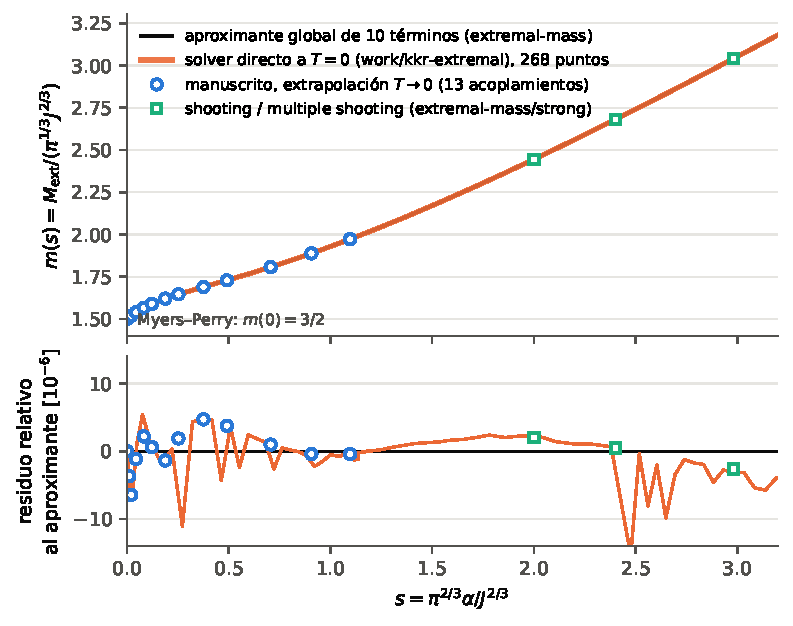
\includegraphics[width=.82\textwidth]{figures/fig-three-routes.pdf}
\caption{Las tres rutas numéricas y el aproximante global; panel inferior, residuos relativos al
aproximante. Los picos de la rama directa en $s>2.3$ son su ruido propio (violaciones de vínculo
$\sim7\times10^{-5}$ en su extremo).}\label{fig:three}\end{figure}
\begin{figure}[t]\centering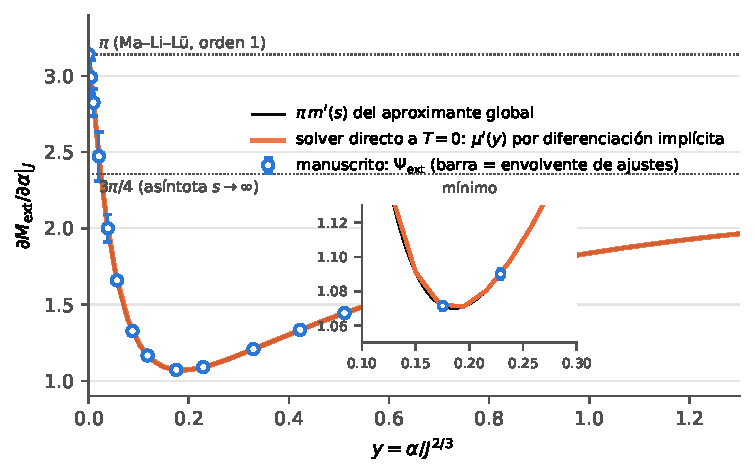
\includegraphics[width=.82\textwidth]{figures/fig-slope.pdf}
\caption{La pendiente $\partial M_\ext/\partial\alpha|_J$ por las tres rutas; recuadro: el mínimo.}
\label{fig:slope}\end{figure}

\subsection{Regeneración de números y suite de tests}
\begin{itemize}
\item \code{manuscript/numbers.tex} se regenera byte a byte con \code{make\_figures.py};
 \code{supplementary/solutions.csv} idéntico; el JSON de sensibilidad difiere en el último bit;
 las 147 macros recomputadas desde \code{results/egb-extremality.json} coinciden (31\,\%, 2.93,
 $4.06\times10^{-6}$, $3.11\times10^{-11}$, $\omega_{\max}=0.762$, etc.).
\item \code{extremal-mass}: \code{make\_numbers.py} regenera \code{numbers.tex} y \code{numerics.tex}
 con \code{diff} vacío; \code{coefficients.json}, \code{gH\_series.json}, \code{c\_constants.json}
 (63 palabras), \code{constants.json} y \code{second\_order\_fields.json} se regeneran idénticos;
 \code{pert.py} a órdenes 2 y 3 reproduce $M_2,M_3,X_2,X_3$ con residuo de primera ley cero;
 $X_5,X_6$ de \code{pert\_order6.json} coinciden con la predicción algebraica de la garganta.
\item Hallazgo positivo: inyectando un valor falso de una constante de horizonte ($C_{011}=-\zeta_3$
 en vez de $-2\zeta_3$), \code{pert.py 3 4} aborta en \code{AssertionError: h not regular}. La
 regularidad en el horizonte está sobredeterminada y detecta una identificación MZV errónea; eso es
 más fuerte que el ``numerical identifications, not proofs'' del README.
\item \code{pytest}: 493/497 aprobados. Fallos: \code{test\_distribution.py} (manifiesto de
 distribución desactualizado, esperado) y
 \code{test\_static\_egb\_bvp.py::test\_spectral\_converges\_with\_resolution}, que pide tolerancia
 $10^{-13}$ y muere en la búsqueda lineal con residuo $1.16\times10^{-13}$: una tolerancia en el
 piso de redondeo que depende de la máquina (mismas versiones de paquetes que producción).
\end{itemize}

\section{Errores y mejoras}
\label{sec:errores}

Severidades: \CRIT{} impide usar el documento tal cual; \MAY{} afirmación falsa o
infundada; \MEN{} inconsistencia o debilidad; \COS{}. ``Ejecutado'' significa que el hallazgo se
reprodujo corriendo algo en esta revisión.

\subsection{Manuscrito (\code{manuscript/main.tex} y acompañantes)}
\label{sec:ms}

\begin{enumerate}[label=M\arabic*.,leftmargin=2.4em]
\item \CRIT{} (ejecutado). \code{main.pdf} (28 páginas, Tectonic, 28/09 23:53) no corresponde al
 \code{main.tex}+\code{numbers.tex} actuales (29 páginas al compilar con la receta de
 \code{build-local.ps1}; 16\,609 vs 17\,701 palabras). Faltan en el PDF, entre otros, los párrafos
 de \code{main.tex} 124--131, 140--151, 1087--1097, 1168--1175, la fila ``radial coordinate'' de la
 tabla de convenciones y el ``Four things would sharpen the result''. \code{README.md} y
 \code{explicacion-en-espanol.md} lo llaman vigente. Esta era la revisión \#1 del informe Codex del
 27/09. Corrección: recompilar y reemplazar; registrar fecha y hash.
\item \MAY{} (ejecutado). Resumen, l.~38--39, y l.~1003--1004: ``the first-order formula overshoots
 the shift by a factor of 1.32''. Con los datos: $\mu_{\rm lin}/\mu=3.8030/2.8885=1.317$, pero
 $\pi y/(\mu-\mu_0)=1.6061/0.6916=2.32$. La macro \code{\textbackslash Nlinearratio} es el cociente
 de masas; la frase habla del desplazamiento. Las diapositivas dicen correctamente ``2.3$\times$''.
 Corrección: ``runs 32\,\% above the extremal mass; the shift itself is overestimated by a factor 2.3''.
\item \MAY{} (ejecutado). Tabla del lugar de cambio de signo, l.~856: encabezado
 ``$\alpha$ \& $x$ \& $t_H$ \& bracket width in $t_H$ \& $j$ \& $q$'' mientras
 \code{make\_figures.py:724-729} genera ``$\alpha$, $x$, $[q_{\rm low},q_{\rm high}]$, $q$, $t_H$, $j$''.
 La fila $\alpha=0$ es \code{0 \& 0.0000 \& [0.63,0.65] \& 0.63474 \& 0.3245 \& 0.9807}: el
 0.63474 es $q$ y el 0.3245 es $t_H$. El PDF enviado tiene el mismo error.
\item \MAY{} (ejecutado). l.~651--658 y 862--864: ``at the other 7 [couplings] no crossing is
 bracketed by accepted solutions and none is reported''. El JSON contiene cruces acotados en
 $\alpha=0.005,\,0.01,\,0.035,\,0.075,\,0.15$ ($q\in[0.63,0.65]$, $[0.65,0.67]$, $[0.69,0.71]$,
 $[0.71,0.73]$, $[0.71,0.73]$); lo que no tienen esas caminatas es cobertura hasta el extremo
 estático. Esto era R10 de la revisión del 25/09; el texto nuevo es ahora directamente falso.
\item \MAY{} (ejecutado). l.~981--984: los incrementos de $\mu$ ``exceed the corresponding spreads
 \ldots by two orders of magnitude or more''. Cocientes incremento/dispersión: 11.7, 19.1, 17.9,
 46.7 en los cuatro primeros acoplamientos, luego $>10^3$.
\item \MEN. Tres entradas de la bibliografía (Myers--Perry 1986, Lovelock 1971,
 Boulware--Deser 1985) no tienen PDF en \code{papers/}, contra la regla de \code{AGENTS.md};
 \code{papers/2607.07418.pdf} está en el archivo y no se cita en ningún lado.
\item \MEN. Apéndice B: definir las $\sigma_i$, los períodos y el mapa a Brihaye et al.\ (4.6):
 $k=2k_{\rm ref}$, $v_3=v_2^{\rm ref}v_3^{\rm ref}$, $J=\partial f/\partial k$ es el $J$ por plano
 ($J_{\rm ref}=2J$); e imprimir $R$ y $\mathcal L_{\rm GB}$ (están en \S\ref{sec:verif}). Son R12 y
 R13 de la revisión anterior, no atendidos.
\item \MEN. l.~112: ``records that the limit could not be reached'' es más fuerte que el original
 de KKR \S3.2 (``The limit is difficult to approach \ldots Nevertheless, we conjecture'').
\item \MEN. l.~1422--1425: la comparación de la ergosuperficie debe dar $r_H=1$, $\Omega_H=0.33$ y
 que la fuente imprime ``$\simeq1.104$'' a tres decimales sin error.
\item \MEN. l.~1716--1725: ``cota superior, la sensibilidad verdadera es menor'' sólo vale sin
 cancelación entre resolución y entorno; decir ``not attributable to resolution alone''.
\item \MEN. Resumen l.~33--34 dice ``a minimum of 1.07'' y el cuerpo ``lowest sampled value''; el
 mínimo continuo sí está resuelto por la rama directa y por el aproximante (\S\ref{sec:tres}):
 $1.070$ en $y\simeq0.19$. Vale la pena citarlo.
\item \COS. Notación con tres usos de $\sigma$, dos de $u$, dos de $f$, dos de $v$; cajas
 \emph{underfull} en l.~395, 413--414, 1932--1937; ruta Windows en \code{check\_manuscript.py:12}.
\item Estado de las revisiones previas: de los 25 ítems del informe del 25/09 están atendidos
 R04, R08, R21 y en gran parte R06 y R23; parciales R01, R03, R05, R07, R11, R12, R15, R16, R25;
 no atendidos R02, R09, R10, R13, R14, R17, R18, R19, R20. De las seis revisiones mayores del
 informe Codex, la \#1 (congelar una versión) sigue abierta y las otras cinco están atendidas o
 parcialmente atendidas.
\item \code{explicacion-en-espanol.md}: habla de ``masa mínima'' y de ``no perturbativo'', dos
 formulaciones que el manuscrito abandonó; su lista de novedades no es la de \code{main.tex}
 167--179. Los números coinciden.
\end{enumerate}

\subsection{Código, tests y reproducibilidad}
\label{sec:code}

\begin{enumerate}[label=C\arabic*.,leftmargin=2.4em]
\item \MAY{} (leído, citado literalmente). Docstrings no corregidos desde R18:
 \code{src/rotating\_bh/extremality.py:6} ``The potential is exact at every point'', \code{:11}
 ``with no step at all'', \code{:18-19} ``reaches $T_H$ of order 1e-5 \ldots at every coupling
 tried'', \code{:23} ``measured twice, independently'', \code{:29} ``share the solver and nothing
 else''; lo mismo en \code{experiments/egb\_extremality.py:15-16,21-22,36,571} y
 \code{extremality\_validation.py:17}. Los datos: $T_{\min}=2.4\times10^{-3}$, $1.2\times10^{-3}$,
 $4.7\times10^{-3}$, $4.0\times10^{-3}$ en $\alpha=0.005$--$0.035$; las dos ``rutas'' comparten
 los mismos seis estados y el mismo ajuste cúbico (\code{extremality.py:283-293}).
\item \MAY{} (ejecutado). \code{tests/test\_near\_horizon.py:86}: umbral
 $10^{-6}\max(1,|f|/\text{step})$ con step $=10^{-6}$, o sea $\approx|f|$. Perturbando $v_2$ un 1\,\%
 el test sigue pasando (derivada $-0.059$ contra umbral $3.38$ en $\tilde\alpha=0.3$). R19 no
 corregido.
\item \MAY{} (ejecutado). Los dos comandos \code{--verify-only} de \code{docs/reproduccion.md:35-36}
 y \code{docs/verificacion.md:16-17} abortan: \code{ValueError: changed numerical input:
 src/rotating\_bh/egb\_rotating\_bvp.py}. Sus \code{verify()} comparan el digest sin consultar
 \code{KNOWN\_EXCEPTIONS} (sólo los tests lo hacen).
\item \MEN{} (ejecutado). \code{test\_spectral\_converges\_with\_resolution} falla en este
 entorno por tolerancia $10^{-13}$ en el piso de redondeo. Subir a $10^{-12}$ o medir
 convergencia, no un residuo absoluto.
\item \MEN. \code{tests/test\_distribution.py} falla en cualquier árbol con trabajo nuevo (404 no
 inventariados: \code{extremal-mass} 384, \code{work/jhep-paper} 9, \code{vault} 3,
 \code{output/pdf} 3, \ldots). Separar la verificación de la distribución congelada de la del árbol
 de trabajo; no regenerar el índice para silenciar.
\item \MEN. La puerta \code{quoted\_bars\_cover\_the\_independent\_route} usa \code{psi\_uncertainty}
 (p.\,ej.\ $2.4\times10^{-3}$ en $\alpha=0.075$) y no la envolvente de 20 ajustes que el paper imprime
 ($2.2\times10^{-2}$); \code{docs/resultados.md:16-18} dice que \code{psi\_uncertainty} no debe
 usarse. Para $\mu$ sólo se usa la dispersión de tres grados (R01 sigue abierto;
 \code{checks/route\_envelopes.py} lo calcula pero no es test).
\item \MEN. \code{extremality.py:204,224}: \code{except Exception} en la caminata convierte
 cualquier bug en ``Newton falló''. \code{egb\_extremality.py:108-140}: caché de progreso sin hash de
 fuentes. Tests tautológicos o de humo con nombres fuertes:
 \code{test\_every\_failing\_gate\_is\_declared}, \code{test\_the\_scalars\_are\_constant\_on\_the\_geometry},
 \code{test\_current\_pdf\_and\_generated\_figures\_are\_present}, \code{test\_environment}.
 Saltos silenciosos si falta un \code{results/*.json}.
\item \MEN. Documentación desactualizada: \code{docs/verificacion.md} (490 tests, 238 hashes, 15
 páginas, 78 macros; hoy 497, 290, 28--29, 147); \code{docs/reproduccion.md:57-60} (``cuatro
 figuras'', dos JSON; son 7 y 4); \code{docs/cambios-tests.md:78} (``byte por byte'' es falso: 7
 tests importan \code{known\_digest\_exceptions}); referencias a archivos inexistentes
 (\code{plans/2026-09-14-hito-8.md}, \code{checks/hito-8.ps1}, \code{reports/originality-precheck.md},
 \code{reports/hito-4*.md}, \code{reports/sdd/task-1-report.md}, \code{project/}); CRLF/LF mixtos;
 rutas Windows en la procedencia.
\item \MEN. \code{AGENTS.md} (vía \code{CLAUDE.md}) describe otro proyecto (``gravitational waves,
 course''), con un layout que el \code{README} no menciona.
\end{enumerate}

\subsection{\code{extremal-mass/}}
\label{sec:em}

\begin{enumerate}[label=E\arabic*.,leftmargin=2.4em]
\item \MAY{} (ejecutado). Radio de convergencia. \code{strong-coupling-report.tex:86-88} y
 \code{extremal-mass-report.tex:51-56} presentan ``signo $d_n=$ signo Re$\,s_*^{-n}$ (6 de 6)'' y
 ``$|d_n||s_*|^n$ decrece lentamente'' como evidencia de que $m(s)$ comparte el radio $0.055$ de
 $g_H$. Con seis coeficientes: $|d_n|^{-1/n}=0.667,0.535,0.351,0.298,0.244$ (sigue bajando);
 el radio implícito de paso dos es $0.39\to0.118$; los cinco signos no triviales sólo acotan el
 argumento de un par dominante a $(75^\circ,90^\circ)$; y $|d_n||s_*|^n$ decrece con factores
 $0.12,0.16,0.56,0.35,0.62$, compatible también con radio $0.09$--$0.1$. La resumación conformal
 no ``sigue la numérica hasta $s\approx0.5$'': $K=6$ queda 1.3\,\% (0.2), 2.9\,\% (0.3) y 6.2\,\%
 (0.5) por debajo, sin oscilar alrededor. Corrección: ``compatible con, no establecido''.
\item \MAY{} (verificado a mano). \code{strong-coupling-report.tex:107-108}: ``the absence of an
 $O(t)$ term means $a_2$ cannot come from the core''. La relación BTZ extremal se asume válida sólo
 al orden dominante; tomada literalmente predice $a_2=0$ y $a_3^{\rm core}=+0.236$, contra
 $a_2=0.4566$, $a_3\simeq-0.263$ de la numérica. La conclusión es cierta por otra vía (el
 \emph{matching}), la inferencia no.
\item \MAY. \code{numerics.tex:24}: ``$m$ independent of the number of far nodes to $5\times10^{-15}$''
 está codificado a mano en \code{make\_numbers.py:114}; \code{ms\_check.json} muestra
 $5.5\times10^{-12}$ (R12 vs R12n40 en $s=48.87$). El $5\times10^{-10}$ (R12 vs R8) sí está
 respaldado.
\item \MEN. Números codificados a mano en \code{make\_numbers.py} (\code{:74,107,113-114}) en vez de
 leídos de sus recibos; ``25.5 min'' es 25.3; ``every point of the earlier spectral branch'' son 11
 puntos muestreados (\code{check\_throat\_vs\_kkr.py:14}); ``all 126 numerical points'' omite que los
 $\sim200$ puntos espectrales con $2<s\le5.24$ se descartaron; el $a_3$ implícito del aproximante es
 $-0.15$, no $-0.26$; con $a_2$ libre los ajustes de 7 términos dan $0.4576$--$0.4579$, así que la
 dispersión sistemática de $a_2$ es $\gtrsim10^{-3}$, no $10^{-4}$.
\item \MEN. \code{check\_c111.py} no hace \code{assert} aunque el README lo presenta como control;
 \code{pert.py:13} dice que las $C_w$ quedan simbólicas y \code{:44-45} las sustituye;
 \code{pert\_order5/6.json} se generaron con Python 3.10 en otra máquina y \code{pert\_order4.json}
 en Windows (el README dice 3.11).
\item \MEN. \code{README.md} y \code{RESUME.txt} desactualizados y contradictorios con los archivos:
 $4/3$ ``candidate'' (confirmado), ``convergence not studied'', tabla sin $d_5,d_6,s_*$, ``NEXT''
 obsoletos, referencias a \code{ms.pid}, \code{ms\_cont.log}, \code{tq\_10.log},
 \code{pert\_order6.log} inexistentes; los tres registros de \code{ms\_results\_v2\_rejected.json}
 llevan \code{"ok": true}; \code{strong\_fit.json} y \code{global\_fit.py} son versiones superadas
 sin nota; $\sim90$\,MB de \code{bvp\_sols*} descartados; 27 scripts de sondeo sin README.
\item \MEN. ``Derived under one assumption'' (\code{extremal-mass-report.tex} \S6) subestima: la
 ruta de \emph{matching} usa cuatro supuestos declarados en el PDF y la ruta BTZ uno; ambas comparten
 la garganta exacta y la hipótesis de núcleo AdS$_3$/BTZ, de modo que ``independent route'' es
 parcial.
\end{enumerate}

\subsection{Documentos secundarios, vault, docs y referencias}
\label{sec:docs}

\begin{enumerate}[label=D\arabic*.,leftmargin=2.4em]
\item \MAY{} (ejecutado). \code{short-summary/summary.tex:239-241} y
 \code{vault/concepts/comparing-against-a-figure-you-cannot-redistribute.md:46}: ``a near-Einstein
 coupling at which our solution is Myers--Perry to thirteen digits''. El control es
 $\alpha_{\rm paper}=0.01$ ($\alpha_{\rm GB}=0.0025$) y allí \code{ours$-$analytic(MP)} llega a
 $6.1\times10^{-3}$ en $h/r^2$; los trece dígitos son el chequeo en $\alpha=0$. El argumento ``the
 departure is not ours'' compara con MP a $\alpha\ne0$, donde MP difiere de la solución en el mismo
 orden ($6\times10^{-3}$) que la discrepancia citada ($9.5\times10^{-3}$). Reescribir.
\item \MAY. \code{vault/papers/arxiv-1201.4994.md:19-22} dice que la entropía exacta de la garganta
 ``would give $\Delta M=J/\sqrt\alpha$ (coefficient 1)'' y que el diccionario BTZ ``does not apply'';
 contradice \code{btz-universality-extremal-egb.md}, ambos reportes y el borrador JHEP ($4/3$,
 verificado aquí). Es un cálculo anterior que quedó sin actualizar.
\item \MAY. \code{reports/kkr-extremal-mass/commentary.html/.pdf} indica reproducir con
 \code{experiments/kkr\_fig1\_extremal\_mass.py}, datos en \code{results/kkr-fig1-extremal-mass.json}
 y ``full version in report.pdf'': ninguno existe. Su afirmación central ($2\times10^{-3}$ en
 $M_\ext$, 0.015 en la pendiente) no es reproducible desde el árbol; además ``reaches $x\approx0.81$''
 está superado por $0.863$.
\item \MAY. \code{README.md:55}: ``Los artículos citados \ldots no se redistribuyen aquí'' mientras
 \code{papers/} contiene 22 PDFs de terceros (21 inventariados en la distribución);
 \code{jheppub.sty} (LPPL) va en el zip de \code{output/pdf} sin mención. \code{references/README.md}
 no existe aunque \code{docs/convenciones.md:7} lo cita; \code{references/sources.json} tiene 4
 entradas, dos sin PDF (0801.1021, 2606.07070) pese a que \code{convenciones.md} se apoya en ellas, y
 no inventaría los otros 20 PDFs.
\item \MAY. Diapositivas y notas (\code{slides-new.tex:174-179,333-336},
 \code{notes-new.tex:204-208}) presentan 36.8\,h / 1.42\,B tokens / 79 prompts como costo del
 proyecto; el libro mayor cierra el 28/09 12:36 y excluye la revisión Codex del 27/09, la
 verificación y la revisión pedagógica del 28/09 y todo octubre (kkr-extremal, extremal-mass, JHEP).
 \code{prompt-log-cronologico.md} tampoco registra los prompts de \code{prompts.txt}.
\item \MEN. Presentación: ``10 independent checks'' (comparten soluciones); notas con ``minimum mass''
 (abandonado en el manuscrito); \code{notes\_ag.tex:54} ``Kerr en 1960'' (1963) y cota atribuida a
 ``$D>4$'' (vale para $D=5$, $J_1=J_2$); \code{questions-answers.tex:408} ``$M=3\pi^2/4(a-c_t)$''
 (KKR (3.15): $M=\tfrac{3\pi}4(a^2-c_t)$); \code{:603-618} alerta sobre líneas del manuscrito que ya
 no existen; \code{slides-new.tex:10} cita \code{v10min/} inexistente.
\item \MEN. Vault: 8 wiki-links sin página (\code{extremality-shift-rotating-black-holes},
 \code{extremal-mass-strong-coupling}, \code{walk-continuation-in-spin},
 \code{rotating-egb-spectral-solver}, \code{boulware-deser-solution},
 \code{external-contrasts-that-do-not-close}, \code{implicit-response-for-psi},
 \code{near-horizon-entropy-function}); \code{vault/templates/} no existe; cuatro páginas huérfanas;
 \code{extremality-shift-pedagogy-revision.md:28} dice que el mínimo en $y\sim0.175$ ``is resolved''
 (contradice al manuscrito y a la rama directa); \code{arxiv-2303.12471.md} cita un directorio
 \code{work/kkr-extremal/arxiv/} inexistente y etiquetas ``at7--at9'' que no están en el PDF.
\item \MEN. \code{work/jhep-paper/main.tex}: números y física correctos contra sus fuentes (verificado
 por compilación y cotejo); ``appendix E'' codificado a mano (l.~208); ``broad minimum'' aunque el
 mínimo continuo está resuelto; el PDF de \code{output/pdf} sí corresponde al fuente.
\item \MEN. \code{verification-report}: ``No external result exists for the rotating mass at finite
 coupling'' contradice a \code{summary.tex:120} (la frontera de KKR lo contiene).
 \code{revision-report} (28/09) describe 25 páginas/128 macros/6 figuras y ``no papers/ directory'',
 superado el mismo día. \code{docs/egb-rotating.md:303-321} vs \code{:438-440}: orientación
 horizonte/infinito contradictoria dentro del mismo archivo.
\end{enumerate}

\subsection{Mejoras recomendadas, por prioridad}

\begin{enumerate}[nosep]
\item Recompilar \code{main.pdf}; corregir M2--M5 (una tarde de trabajo, todo son frases y un
 encabezado); añadir los tres PDFs faltantes a \code{papers/} o anotar la excepción.
\item Reescribir los docstrings C1, arreglar el test C2 (comparar derivadas por paso complejo con
 las expresiones generadas, con un control negativo), y hacer que los \code{verify()} de C3 consulten
 las excepciones conocidas.
\item Rebajar la retórica del radio de convergencia (E1) y de la inferencia sobre $a_2$ (E2);
 reemplazar el $5\times10^{-15}$ (E3) por el valor del recibo; actualizar README y RESUME de
 \code{extremal-mass} con un ``estado final'' al principio.
\item Corregir D1--D5 (una frase falsa, una página de vault, un reporte huérfano, dos párrafos de
 licencias/referencias, una nota de alcance en las diapositivas).
\item Incorporar al manuscrito la validación cruzada de \S\ref{sec:tres}: es un argumento más fuerte
 que las envolventes de ajuste, y ya está hecho (rama directa en \code{work/kkr-extremal}).
\item Separar el verificador de distribución del árbol de trabajo; registrar el entorno de
 \code{.venv} (3.11.18) en \code{docs/}; unificar la fecha/alcance del libro mayor de tokens.
\end{enumerate}

\section{¿Es factible una expresión analítica para la masa extremal?}
\label{sec:analitica}

\subsection{Lo que se sabe exactamente}

Por escala, $M_\ext=\pi^{1/3}J^{2/3}m(s)$ con $s=\pi^{2/3}\alpha/J^{2/3}$ (equivalentemente
$\mu(y)=\pi^{1/3}m(\pi^{2/3}y)$), y $\partial M_\ext/\partial\alpha|_J=\pi m'(s)$. Se dispone de:
\begin{itemize}
\item \textbf{Serie débil exacta a orden 6}:
 $m=\tfrac32+s-\tfrac{236}{105}s^2+d_3s^3+\dots+d_6s^6$, con $d_3=\tfrac{60851752}{33075}-1536\zeta_3$,
 $d_4=-\tfrac{592541765354296}{1489863375}+\tfrac{227328}5\zeta_3+\tfrac{88064}{25}\pi^4$, y $d_5,d_6$
 con $\zeta_5$, $\zeta_3^2$, $\zeta_2^3$ (valores en \code{series/coefficients.json}). Condicional a
 la identificación PSLQ de constantes de horizonte, pero esa identificación está sobredeterminada por
 la regularidad (\S\ref{sec:verif}) y los corrimientos racionales $X_5,X_6$ coinciden con la garganta.
\item \textbf{Garganta algebraica a todo acoplamiento}, rederivada aquí: $P(a,q)=0$,
 $8J^2/(\pi^2g_H^3)=q^2(4-q)[1+4a(4-3q)]/8$, $S_\ext=\tfrac{\pi^2}2g_H^{3/2}\sqrt q\,[1+4a(4-q)]$.
 A $J$ fijo da $g_H(s)$, $q(s)$, $S_\ext(s)$ exactos. No da la masa: la normalización asintótica
 del tiempo no es un dato de la garganta.
\item \textbf{Acoplamiento fuerte}: $m=\tfrac34s+\tfrac43s^{-1/2}+a_2s^{-1}+a_3s^{-3/2}+\dots$, con
 $4/3$ derivado bajo la hipótesis del diccionario BTZ para el núcleo rotante y confirmado a
 $4\times10^{-4}$; $a_2=0.456527$ condicional (numérico $0.4566\pm0.0002$); $a_3\simeq-0.263$ numérico.
\item \textbf{Identidades exactas}: Smarr a $T=0$, $M_\ext=3\Omega_HJ+\alpha\,\partial_\alpha M_\ext|_J$,
 es decir $3\Omega_HJ^{1/3}=\mu-y\mu'$; primera ley $\partial_JM_\ext|_\alpha=2\Omega_H$.
\item \textbf{Aproximante global} (\S\ref{sec:english}, ec.~\eqref{eq:approx}): exacto en ambos
 extremos, error $1.1\times10^{-5}$ en $0<s\le103$.
\end{itemize}

\subsection{Por qué una forma cerrada no es factible hoy}

\begin{enumerate}
\item Los $d_n$ contienen valores zeta múltiples de peso hasta $n$. Una función algebraica de $s$
 sobre $\mathbb Q$, o hipergeométrica en $s$ con parámetros racionales, tiene coeficientes
 racionales; los zeta de peso creciente aparecen cuando $s$ entra en los \emph{parámetros}
 (típicamente funciones $\Gamma$ de exponentes que dependen de $s$, y la garganta tiene un exponente
 exacto e irracional $\gamma(s)$). Cualquier forma cerrada sería no elemental, con $s$ en exponentes.
\item La serie tiene singularidades complejas cerca del origen (conjeturalmente $s_*$, radio
 $0.055$; en cualquier caso radio $\lesssim0.12$) y en $s\to\infty$ cambia a una expansión en
 $s^{-1/2}$ tras un término lineal. La sesión anterior descartó superpotenciales de
 Hamilton--Jacobi con Laurent finito, soluciones liouvillianas de la ecuación de \emph{squashing}
 (grupo de Galois $SL(2,\mathbb C)$) y una ODE candidata resonante.
\item \textbf{Intento nuevo de esta revisión} (\code{checks/uniformize\_q.py}): como $s_*$ es un
 punto crítico del mapa algebraico $s(q)$, en la variable $q=h_H/g_H$ el pliegue desaparece y ambos
 extremos son series en $q$. Compuse la serie exacta con $s(q)$ y expandí $y=m-3s/4$ en $w=2-q$:
 $y=\tfrac32+0.03125w-0.05595w^2+0.10348w^3-0.26867w^4+0.65415w^5-1.80098w^6+\dots$ Los
 coeficientes crecen con razón $\approx-2.6$ (radio $|w|\approx0.4$), y el discriminante exacto
 $D(q)=5q^4-34q^3+73q^2-56q+16$ se anula en $q=2.2763$, $|2-q|=0.276$: sobre la rama continuada a
 acoplamiento negativo $q$ tiene un extremo allí, así que $q$ no uniformiza cerca de Myers--Perry.
 Contra la numérica, la serie en $w$ es \emph{peor} que la serie en $s$ ($2.6\times10^{-3}$ frente a
 $7.5\times10^{-6}$ en $s=0.044$) y un Padé $[3/3]$ en $w$ falla más allá de $s\approx0.05$. Un Padé
 $[3/3]$ de $m(s)$ sólo extiende el rango útil hasta $s\approx0.4$ (error $5\times10^{-3}$) y es
 inútil más allá de $s\approx0.7$. Resultado negativo, documentado con recibo.
\end{enumerate}

\subsection{Respuesta}

No se encontró ni es factible, con lo que hay, una expresión cerrada de $M_\ext(J,\alpha)$. La
``expresión analítica'' disponible es el par de expansiones exactas en los dos extremos más la
garganta algebraica, y para uso práctico el aproximante global. Los caminos que podrían cambiar la
respuesta (derivar $a_2$ exactamente; uno o dos órdenes más de la serie para fijar el radio;
buscar una estructura resumada en la que $s$ entre a través de $\gamma(s)$; probar que $m(s)$ hereda
el pliegue de la garganta) son tareas de semanas y ninguna garantiza una forma cerrada. El reporte
en inglés que sigue reúne todo esto en forma autocontenida.

\clearpage
\section{Report in English: the search for an analytic expression of the extremal mass}
\label{sec:english}
\selectlanguage{english}
% Body of the English report on the analytic expression. Included by review-report.tex and by
% analytic-expression-report.tex (standalone).

\subsection*{Question}

Is there an analytic expression for the extremal mass $M_{\rm ext}(J,\alpha)$ of the
five-dimensional, asymptotically flat, equal-spin ($J_1=J_2=J$) Einstein--Gauss--Bonnet black
hole, action $(16\pi G_5)^{-1}\!\int\!\sqrt{-g}\,(R+\alpha\mathcal L_{\rm GB})$, $G_5=1$?
Scale invariance reduces the problem to one function of one variable,
\begin{equation}
 M_{\rm ext}=\pi^{1/3}J^{2/3}\,m(s),\qquad s=\frac{\pi^{2/3}\alpha}{J^{2/3}},
 \qquad\text{equivalently}\qquad \mu(y)=\frac{M_{\rm ext}}{J^{2/3}}=\pi^{1/3}m(\pi^{2/3}y),\ \ y=\frac{\alpha}{J^{2/3}},
\end{equation}
and the slope studied in the manuscript is $\partial M_{\rm ext}/\partial\alpha|_J=\mu'(y)=\pi\,m'(s)$.

\subsection*{Short answer}

A closed form for $m(s)$ is not available and, on the present evidence, is not feasible with
the tools used in this project. What \emph{is} established, and what this review verified
independently, is an exact description of both ends of the function and of the near-horizon
data at every coupling, together with a global representation accurate to $10^{-5}$. No new
closed form was found here; one further natural attempt (expansion in the algebraic throat
variable) was made and is reported below as a negative result.

\subsection*{What is known exactly}

\paragraph{Weak coupling.} The project's exact exterior solver (\texttt{extremal-mass/code/pert.py})
gives, with $\zeta_n=\zeta(n)$,
\begin{align}
 m(s)&=\tfrac32+s-\tfrac{236}{105}s^2+d_3s^3+d_4s^4+d_5s^5+d_6s^6+\dots,\\
 d_3&=\tfrac{60851752}{33075}-1536\,\zeta_3=-6.548307\ldots,\qquad
 d_4=-\tfrac{592541765354296}{1489863375}+\tfrac{227328}{5}\zeta_3+\tfrac{88064}{25}\pi^4=66.100522\ldots,\nonumber\\
 d_5&=\tfrac{447853140007115845664}{6100990520625}+\tfrac{657983488}{175}\zeta_3-\tfrac{3972366336}{625}\zeta_2^2-\tfrac{1464139776}{25}\zeta_5\nonumber\\&=423.920197\ldots,\nonumber\\
 d_6&=-4737.494827\ldots\ \ (\text{exact form in \texttt{extremal-mass/series/coefficients.json}}).\nonumber
\end{align}
The first two terms are the published result of Ma, Li and L\"u. The coefficients are exact
conditional on the identification (PSLQ at 100 digits) of regularised horizon constants with
multiple zeta values; the audit found that this identification is over-determined by the
horizon-regularity conditions of the solver (injecting a wrong value for one constant makes the
order-3 run abort with ``$h$ not regular''), and the rational horizon shifts $X_5,X_6$ coincide with
an independent algebraic prediction. The series is therefore trustworthy. Its radius of
convergence is small: the throat data have a square-root branch point at
$s_*=0.00592\pm0.05482\,i$, $|s_*|=0.0551$; the six known $d_n$ are compatible with, but do not
establish, the same radius for $m(s)$ (the ratio test on six terms only bounds it by roughly
$0.12$).

\paragraph{Near-horizon data at any coupling.} Writing $g_H=r_H^2$, $a=\alpha/g_H$ and
$q=h_H/g_H$ for the horizon squashing, Sen's entropy function on the throat
$\mathrm{AdS}_2\ltimes S^3$ gives (rederived here from scratch, 12 assertions in
\texttt{checks/check\_throat2.py})
\begin{gather}
 16a^2q^2(4-q)-8a(2q^2-7q+4)+q-2=0,\qquad
 \frac{8J^2}{\pi^2g_H^3}=\frac{q^2(4-q)\,[1+4a(4-3q)]}{8},\label{eq:throat}\\
 S_{\rm ext}=\frac{\pi^2}{2}\,g_H^{3/2}\sqrt q\,\bigl[1+4a(4-q)\bigr],\nonumber\\
 v_1=\frac{(1+4aq)(12aq-16a-1)}{4(6aq^2-16aq-1)},\qquad
 e^2=\frac{(q-4)(1+4aq)^2(12aq-16a-1)}{4q\,(6aq^2-16aq-1)^2},\nonumber
\end{gather}
with $v_1$ the $\mathrm{AdS}_2$ radius squared and $e$ the fibre electric field. At fixed $J$
these equations determine $g_H(s)$, $q(s)$ and $S_{\rm ext}(s)$ as algebraic functions. They do
\emph{not} determine the mass: $M_{\rm ext}$ needs the asymptotic normalisation of the time
coordinate, which the throat discards. (Equation (3.18) of Kleihaus--Kunz--Radu prints the total
$J_1+J_2$; the project's per-plane normalisation is the consistent one.)

\paragraph{Strong coupling.} Matched asymptotics and, independently, a BTZ dictionary for the
small-$r$ core of static EGB black holes give
\begin{equation}
 m(s)=\frac{3s}{4}+\frac43\,s^{-1/2}+a_2\,s^{-1}+a_3\,s^{-3/2}+\dots,\qquad
 M_{\rm ext}=\frac{3\pi\alpha}{4}+\frac{4J}{3\sqrt\alpha}+a_2\frac{J^{4/3}}{\pi^{1/3}\alpha}+\dots
\end{equation}
The leading term is the mass of the nakedly singular static solution (the endpoint conjectured
by Kleihaus, Kunz and Radu); $a_1=4/3$ is derived under the assumption that the rotating
extremal core obeys the static BTZ dictionary and is confirmed numerically to $4\times10^{-4}$;
$a_2=0.456527$ is a conditional analytic value, numerically $0.4566\pm0.0002$; $a_3\simeq-0.263$
is purely numerical. The audit noted that the BTZ relation, taken literally beyond leading
order, would give $a_2=0$, so the dictionary is a leading-order statement only.

\paragraph{Exact identities that constrain any candidate.} The Smarr relation at $T=0$ gives
$M_{\rm ext}=3\Omega_HJ+\alpha\,\partial M_{\rm ext}/\partial\alpha|_J$, i.e.
$3\,\Omega_HJ^{1/3}=\mu-y\mu'$, so the minimum of the slope is the maximum of the scaled horizon
angular velocity; the first law at $T=0$ gives $\partial M_{\rm ext}/\partial J|_\alpha=2\Omega_H$.
Both hold on all three numerical branches checked here.

\subsection*{Numerical knowledge, cross-validated}

Three independent determinations exist in the repository: the manuscript's zero-temperature
extrapolation of non-extremal solutions (13 couplings, $s\le1.10$), the direct $T=0$ spectral
solver of \texttt{work/kkr-extremal} ($s\le5.2$), and the shooting / multiple-shooting branch
of \texttt{extremal-mass/strong} ($2\le s\le103$). This review compared them with each other,
with the exact series and with the ten-term global approximant (table~\ref{tab:threeroutes},
figures~\ref{fig:three}--\ref{fig:slope}): $m$ agrees to $6\times10^{-6}$ relative across all
sources, the slope to $3\times10^{-4}$ (within the manuscript's own fit envelopes), and the
minimum of the slope is $\partial M_{\rm ext}/\partial\alpha|_J\simeq1.070$ at
$y\simeq0.19$ ($s\simeq0.40$) on every route. The approximant
\begin{equation}
 m(s)\simeq\frac{3s}{4}+\sum_{k=1}^{10}c_k\,t^k,\qquad t=\Bigl(1+\frac s\kappa\Bigr)^{-1/2},\quad
 \kappa=0.356242695,
 \label{eq:approx}
\end{equation}
with
\begin{equation*}
\begin{aligned}
 c_{1\ldots5}&=2.233910,\ 1.281505,\ -0.713812,\ 6.055449,\ -75.189708,\\
 c_{6\ldots10}&=230.148117,\ -352.252482,\ 303.906361,\ -142.214324,\ 28.244984,
\end{aligned}
\end{equation*}
reproduces $m(0)=3/2$, $m'(0)=1$,
$a_1=4/3$, $a_2=0.456527$ exactly and every numerical point to $1.1\times10^{-5}$. It is the
best available ``expression'' for practical use, but it is an interpolant: its Taylor
coefficients beyond $s^1$ and its $s^{-3/2}$ coefficient ($-0.15$ instead of $-0.26$) are not
those of $m(s)$.

\subsection*{Why a closed form is unlikely, and what was tried}

\begin{enumerate}
\item \textbf{Transcendental structure.} $d_n$ contains multiple zeta values of weight up to $n$
 ($\zeta_3$ at order 3, $\zeta_2^2$ at order 4, $\zeta_5$ at order 5, $\zeta_3^2$ and
 $\zeta_2^3$ at order 6). An algebraic function of $s$ over $\mathbb Q$, or a hypergeometric-type
 function of $s$ with rational parameters, has rational Taylor coefficients. Zeta values of
 growing weight arise instead when the \emph{parameters} of such functions depend on $s$,
 for instance through $\Gamma$-functions of the throat exponent $\gamma(s)$, which is exact
 and irrational ($\lambda^2+\lambda=Q(a,q)$ in the project's endpoint report). Any closed form
 would therefore have to be non-elementary, with $s$ entering through exponents.
\item \textbf{Singularities.} The weak series has complex singularities close to the origin
 (conjecturally $s_*$, radius $0.055$); the function has an essential change of behaviour at
 $s\to\infty$ (expansion in $s^{-1/2}$ after a linear term). A simple formula interpolating the
 two ends and respecting $s_*$ was sought by the previous session without success
 (finite-Laurent Hamilton--Jacobi superpotentials, Liouvillian solutions of the squashing
 equation --- its Galois group is $SL(2,\mathbb C)$ --- and a resonant candidate ODE for $m(s)$,
 all ruled out).
\item \textbf{New attempt in this review: the throat variable.} Since $s_*$ is a critical
 point of the exact algebraic map $s(q)$, the fold disappears in the variable $q$; both ends of
 the branch are series in $q$ ($q\to2$ at Myers--Perry, $q\to0$ at strong coupling, with
 $s^{-1/2}\propto q$ there). We composed the exact series with $s(q)$ and expanded
 $y(q)=m-3s/4$ in $w=2-q$:
 $y=\tfrac32+0.03125\,w-0.05595\,w^2+0.10348\,w^3-0.26867\,w^4+0.65415\,w^5-1.80098\,w^6+\dots$
 The coefficients grow geometrically with ratio $\approx-2.6$, i.e.\ radius $|w|\approx0.4$, and
 the exact discriminant $D(q)=5q^4-34q^3+73q^2-56q+16$ of the throat vanishes at $q=2.2763$,
 $|2-q|=0.276$: on the branch continued to negative coupling $q$ has an extremum there, so $q$
 is not a uniformising coordinate near Myers--Perry. Against the numerics the $w$-series is
 \emph{worse} than the $s$-series (error $2.6\times10^{-3}$ at $s=0.044$ versus
 $7.5\times10^{-6}$), and a $[3/3]$ Pad\'e in $w$ fails beyond $s\approx0.05$. A $[3/3]$ Pad\'e
 of $m(s)$ itself extends the useful range only to $s\approx0.4$ (error $5\times10^{-3}$) and
 is useless beyond $s\approx0.7$. Negative result; receipts in
 \texttt{checks/receipts/uniformize\_q.txt}.
\end{enumerate}

\subsection*{What would move the question}

(i) An exact derivation of $a_2$ from the next order of the core/intermediate matching, which
would fix the strong-coupling side to two exact terms; (ii) one or two more exact orders
$d_7,d_8$ (the solver scales badly: order 6 took 1\,h\,38\,min and 200\,MB) to test the
conjectured radius $|s_*|$ and the large-order form $d_n\sim2\,\mathrm{Re}[C\,s_*^{-n}n^{\beta}]$;
(iii) a search for a resummed structure in which $s$ enters through the exact throat exponent
$\gamma(s)$, e.g.\ ratios of $\Gamma$-functions reproducing the weight pattern of the $d_n$;
(iv) a proof, from the horizon expansion in $r^{2\gamma}$, that $m(s)$ inherits the throat fold.
None of these is a small task, and none is guaranteed to yield a closed form. Until then the
honest statement is: $M_{\rm ext}(J,\alpha)$ is known exactly as two asymptotic expansions, its
near-horizon data are algebraic at every coupling, and the function in between is known
numerically to $10^{-5}$ and summarised by eq.~\eqref{eq:approx}.

\selectlanguage{spanish}

\clearpage
\appendix
\section{Archivos creados por esta revisión}

Todo está bajo \code{review-claude-2026-10-27/}; nada del proyecto fue modificado (sí se creó
\code{.venv}, que \code{.gitignore} excluye, y se instaló \code{uv} en \code{\textasciitilde/.local/bin}).
\begin{itemize}[nosep]
\item \code{checks/check\_thermo.py}: 42 aserciones de termodinámica, convenciones y soluciones exactas.
\item \code{checks/check\_throat2.py}: función de entropía de Sen sobre la garganta, 12 aserciones.
\item \code{checks/check\_branch\_consistency.py}: cotejo de las tres rutas numéricas, la serie y el
 aproximante; escribe \code{branch\_consistency.json}.
\item \code{checks/uniformize\_q.py}: reexpansión en la variable de garganta, Padés; escribe
 \code{uniformize\_q.json}.
\item \code{checks/make\_figures.py}: figuras del reporte.
\item \code{checks/receipts/*.txt}: salidas íntegras de cada script, de \code{pytest} y del entorno.
\item \code{report/review-report.tex/.pdf} (este documento) y
 \code{report/analytic-expression-report.tex/.pdf} (el reporte en inglés, también autocontenido).
\item \code{vault/exercises/review-2026-10-27.md}: página de vault con el recibo de ejecución.
\end{itemize}

\section{Recibos de ejecución (extractos)}
\small
\begin{verbatim}
$ .venv/bin/python checks/verify_recorded_digests.py
OK: available inputs match, apart from the explicitly listed exceptions   (290 digests, 7 exceptions)
$ .venv/bin/python manuscript/check_manuscript.py
ok: 147 generated quantities, 20 references, no literal numbers in the body
$ .venv/bin/python checks/verify_distribution.py
438 distribution files; 405 failures   (404 unlisted, 1 changed: .gitignore, 0 missing)
$ OPENBLAS_NUM_THREADS=1 .venv/bin/python -m pytest -q
FAILED tests/test_distribution.py::test_published_distribution_is_intact
FAILED tests/test_static_egb_bvp.py::test_spectral_converges_with_resolution
   -> SolverFailure: spectral line search failed; residual=1.16282e-13
2 failed, 493 passed, 2 skipped in 657.96s
$ .venv/bin/python -B review-claude-2026-10-27/checks/check_thermo.py
42 assertions passed; 6 of them certified numerically at random rational points (60 digits)
$ .venv/bin/python -B review-claude-2026-10-27/checks/check_throat2.py
R = e**2*v3/(2*v1**2) + 8/v2 - 2*v3/v2**2 - 2/v1
third equation -> -6*pi*(4*a*q + 1)*(12*a*q - 16*a - 1)*(16*a**2*q**3 - 64*a**2*q**2
                  + 16*a*q**2 - 56*a*q + 32*a - q + 2)
12 assertions passed in 41 s
$ .venv/bin/python -B review-claude-2026-10-27/checks/check_branch_consistency.py
worst |m_manuscript - m_series6|/m for s < 0.055 : 4.89e-06
worst |m_manuscript - m_approximant|/m        : 6.43e-06
worst |Psi_manuscript - pi m'_approximant|     : 2.13e-03
worst |mu_manuscript - mu_spectral| (interp)   : 2.38e-05
worst |Psi_manuscript - Psi_spectral| (interp) : 2.98e-04
approximant: min of Psi = pi m'(s) = 1.07000 at s = 0.39770, y = 0.18541
spectral branch: quadratic fit minimum 1.06976 at y = 0.19527
Environment: Python 3.11.18, numpy 2.4.6, scipy 1.17.1, sympy 1.14.0, mpmath 1.3.0,
matplotlib 3.11.1; pdfTeX 3.141592653-2.6-1.40.22 (TeX Live 2022); Linux 5.15.0-179 x86_64.
\end{verbatim}
\end{document}
